% !TEX TS-program = XeLaTeX
%twocolumn

\documentclass[aimcpersian]{aimc46}
\title{تهدیدات امنیتی خانه هوشمند در لایه اشیا و راه های مقابله با آن ها}
\author{
زهرا دهقانیان%
\RTLthanks{ارایه دهنده}\index{دهقانیان، زهرا}
\university{دانشجوی نرم افزار دانشگاه امیرکبیر}
\and
دکتر رضا صفابخش
\index{صفابخش،رضا}\university{استاد دانشگاه امیرکبیر}
}

\begin{document}
\pagestyle{plain}
\maketitle

\begin{abstract}
  اینترنت اشیاء بستری است که در آن شبکه اینترنت موجود از سیستم‌های رایانه‌ای به اشیاء یا موجودیت‌های دنیای واقعی متصل هستند؛ اشیاء ممکن است شامل موجودیت‌ها، وسایل برقی خانگی، دستگاه‌ها، ابزار، وسایل اسباب‌بازی و هر وسیله‌ای که قابلیت متصل شدن به اینترنت را داشته باشد. این اشیاء طبق زیرساخت مشخص و پروتکل‌های استاندارد خاصی به اینترنت متصل شده و اینترنت اشیاء شکل می‌گیرد. اشیاء در اینترنت هوشمند می‌توانند حقیقی یا مجازی و ثابت یا متحرک باشند. اشیاء، می‌توانند با یکدیگر و با انسان تعامل داشته باشند که این ارتباطات به ترتیب، ارتباط شی به شی و ارتباط شی با انسان نامیده می‌شوند. از حوزه‌های اینترنت اشیاء می‌توان به حوزه‌ نقل ‌و انتقال هوشمند، درمان هوشمند، کشاورزی هوشمند، خانه هوشمند، وسایل نقلیه هوشمند، مدرسه هوشمند، بازار هوشمند، و صنعت هوشمند نام برد. در این تحقیق ما به تهدیدات امنیتی حانه هوشمند پرداخته و برای امن‌سازی این تهدیدات راهکارهای مناسب ارایه می‌دهیم.
\end{abstract}
\keywords{اینترنت اشیاء، خانه هوشمند، تهدیدات امنیتی، امن‌سازی}

%\twocolumn

\section{مقدمه }
    اینترنت اشیا یا $IOT$\LTRfootnote{Internet Of Things} بخشی از اینترنت آینده است که شامل اینترنت موجود و در حال رشد و همچنین توسعه‌های آینده شبکه می شود. اینترنت اشیا به طور مفهومی می تواند به عنوان یک زیر ساخت شبکه سراسری پویا با قابلیت های خود پیکربندی و مبتنی بر استانداردها و پروتکل های ارتباطی جمعی و مشارکتی تعریف شود که در آن "اشیا" فیزیکی و مجازی دارای شناسه‌ها، صفات فیزیکی و مشخصه های مجازی، از واسطه های هوشمند استفاده کرده و به طور یکنواخت و مستمر در یک شبکه اطلاعات مجتمع شده اند. مساله امینت در $IOT$ را می ‌توان مهم‌ترین چالش توسعه این فناوری در نظر گرفت. در این رابطه استانداردهای مختلفی در حال توسعه است؛ ولی همچنان نیازمندی های امنیتی اینترنت اشیا و حتی مخاطرات آن به خوبی شناسایی و تحلیل نشده است.   اینترنت اشیاء بستری است که در آن شبکه اینترنت موجود از سیستم‌های رایانه‌ای به اشیاء یا موجودیت‌های دنیای واقعی متصل هستند؛ اشیاء ممکن است شامل موجودیت‌ها، وسایل برقی خانگی، دستگاه‌ها، ابزار، وسایل اسباب‌بازی و هر وسیله‌ای که قابلیت متصل شدن به اینترنت را داشته باشد. این اشیاء طبق زیرساخت مشخص و پروتکل‌های استاندارد خاصی به اینترنت متصل شده و اینترنت اشیاء شکل می‌گیرد. اشیاء در اینترنت هوشمند می‌توانند حقیقی یا مجازی و ثابت یا متحرک باشند. اشیاء، می‌توانند با یکدیگر و با انسان تعامل داشته باشند که این ارتباطات به ترتیب، ارتباط شی به شی و ارتباط شی با انسان نامیده می‌شوند. از حوزه‌های اینترنت اشیاء می‌توان به حوزه‌ نقل ‌و انتقال هوشمند، درمان هوشمند، کشاورزی هوشمند، خانه هوشمند، وسایل نقلیه هوشمند، مدرسه هوشمند، بازار هوشمند، و صنعت هوشمند نام برد. سیستم خانه هوشمند می‌تواند همانند آنچه در تصویر زیر نشان داده شده، پیکربندی شود؛ سیستم خانه هوشمند شامل سه مؤلفه اصلی سرور خانه، دروازه خانه و دستگاه‌های خانه هوشمند است

\section{مرور سوابق و پیشینه}
اینترنت اشیا توسط فن‌آوری ناهمگن ایجاد می‌شود که موفق به تأمین خدمات نوآورانه در حوزه های مختلف نرم‌افزار است. در این سناریو، رضایت از امنیت و حریم خصوصی نقش اساسی مورد نیاز بازی می‌کند. محرمانه بودن اطلاعات و احرازهویت، کنترل دسترسی در شبکه اینترنت اشیا، حفظ حریم خصوصی و اعتماد در میان کاربران از اهمیت زیادی برخوردار است، بنابر این در حوزه فعالیت‌های تحقیقاتی زیادی انجام گرفته و مقالات فراوانی نوشته شده است، که به برخی از آنها اشاره می‌شود. آقای رسلین و همکاران\cite{M1} در مقاله خود تهدیدات امنیتی خانه هوشمند را بررسی کرده است. بنگالی و همکاران\cite{M2} با استفاده فناوری$GSM$ امنیت خانه هوشمند را بررسی و راهکارهای امنیتی مرتبط را ارایه کرده است. 
توسعه دستگاه‌ها و سرویس‌های خانه هوشمند توسط فروشندگان دستگاه و تأمین‌کنندگان خدمات: در طول این فاز، فروشندگان و تأمین‌کنندگان خدمات، نیازمندیهای محصول، طراحی، توسعه و تست محصول را تعریف می‌کنند. 
بهره‌مندی از دستگاه‌ها و سرویسها تا پایان حیات آنها: کاربر نهایی فارغ از تعاملات مستقیم و محلی با دستگاه خود، از فروشنده درخواست حمایت کرده و از سرویسهای برخط مرتبط با دستگاه از طریق کانالهای ارتباطی مختلف استفاده می‌کند بنابراین شاید این فاز بر تعاملات با فروشنده دستگاه، تأمین‌کننده سرویس یا تأمین‌کننده خدمات الکترونیکی برای استفاده و انهدام دلالت دارد.

\section{طرح پیشنهادی}

سیستم خانه هوشمند مطابق شکل\ref{Home} می‌تواند پیکربندی شود، سیستم خانه هوشمند شامل سه مؤلفه اصلی سرور خانه، دروازه خانه و دستگاه‌های خانه هوشمند است.
ابتدا سرور‌خانه فرآیندهای ذخیره‌سازی، تجمیع و توزیع اطلاعات گردآوری شده از رسانه‌های مختلف موجود در خانه را انجام می‌دهد، سپس دروازه‌خانه، صاحب شبکه دسترسی را به شبکه خانگی متصل می‌کند؛ در نهایت دستگاه‌های خانه هوشمند قادر خواهند بود اطلاعات را میان دستگاه‌ها مبادله کرده و به اینترنت خارجی نیز دسترسی پیدا کند. 
مؤلفه‌های تشکیل‌دهنده سیستم خانه هوشمند در مواجهه با تهدیدات داخلی یا خارجی قرار دارند زیرا اغلب این مؤلفه‌ها به اینترنت متصل هستند؛ برای غلبه بر چنین تهدیدات امنیتی، مانند تزریقات بدافزاری، دسترسی احراز هویت شده کاربر، افشای اطلاعات اساسی، لازم است تمهیدات امنیتی مطابق بر مشخصه‌های مؤلفه‌ای سیستم خانه هوشمند به کار گرفته شود. استفاده از مکانیزمهای امنیتی اختصاصی بسته به راه‌حل استفاده شده تغییر می‌یابد؛ چندین روش از لایه انتقال به لایه کاربرد به کار گرفته می‌شوند.

\begin{figure}[h]
\centering
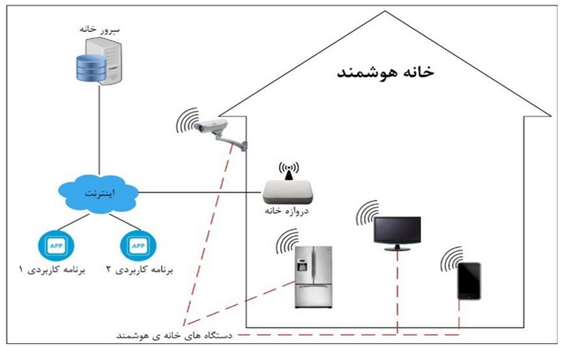
\includegraphics[width=13cm]{figures/Home.png}
\caption{سیستم خانه هوشمند}
\label{Home}
\end{figure}



•	پروتکلهای احراز هویت ـ اعتبارسنجی کاربر، مانند $Oauth/OpenID، XACML/SAML$، ثبت‌نام و غیره

•	پروتکل حفاظت از ارتباط مانند $SSL/TLS$ در سرتاسر $TCP/IP$، یا $DTLS$ در طول $UDP$ 

•	استفاده از الگوریتمهای رمزنگاری برای امن کردن لایه انتقال، که در میان شمار تعدادی از پروتکلهای ارتباطی یافت می‌شود.
 

\subsection{تهدیدات خانه هوشمند}

خانه‌های هوشمند از مؤلفه‌های متعددی تشکیل شده‌اند؛ این مؤلفه‌ها همواره در معرض تهدیدات مختلفی قرار دارند. حملات خانه‌های هوشمند به هفت گروه تقسیم شده‌اند که عبارتند از:
 \begin{enumerate}
 \item
\textbf{ 	حملات فیزیکی:} به دستکاری فیزیکی دستگاه‌ها اطلاق می‌شود؛ این حملات می‌تواند به انواع مختلفی از خطرات مانند فعالیت، سوءاستفاده نابهنجار یا استراق سمع، ممانعت یا سرقت منجر شود؛ معمولا یک حمله فیزیکی تمامی اموال را تحت تأثیر قرار می‌دهد.
 \item
 \textbf{	خسارات ناخواسته (تصادفی): }ممکن است از اطمینان نادرست و نابجا به افراد و آشنایان یا اشتباهات شخصی (مدیریتی، طراحی، عملکرد وغیره) ناشی شود؛ می‌تواند مراتب جبران ناپذیری همچون نشر اطلاعات، تغییرات غیرمعتبر یا حتی فقدان اطلاعات را با خود به همراه داشته باشد. 
 \item
 \textbf{	فجایع و قطع برق:} انکار خدمات برای کاربر را با خود به همراه دارد.
  \item
 \textbf{		آسیب  و فقدان:} نه تنها منجر به تخریب سرویس می‌شود، بلکه نشر اطلاعات را با خود به همراه دارد؛ در واقع باعث حذف اطلاعات حیاتی می‌شود.
 \item
 \textbf{		خرابیها و بد عملکردها:} مهمترین نقطه شروع حمله توسط مهاجم است؛ مهاجم با بهره‌جویی از این فرصت، مبادرت به فعالیت، سوءاستفاده نابهنجار و استراق سمع، ممانعت و سرقت می‌کند.
 \item
 \textbf{		استراق سمع، ممانعت و سرقت:} سوءاستفاده ناهنجار به تهدیدات سایبری و نیز حریم شخصی مربوط می‌شود؛ این دو مقوله به عنوان تهدیدات امنیتی در نظر گرفته می‌شود؛ مهاجم با تغییر طراحی یا به کارگیری نواقص، یک یا چند دارایی و موجودیت را به خطر خواهد انداخت که در نتیجه منجر به نقض محرمانگی داده‌های خصوصی یا از دست دادن کنترل یک دستگاه خواهد شد.
 \item
 \textbf{		قانونی:} این نوع تهدید مراتبی همچون تهدیدات گذشته خواهد داشت اما نسبت به سایر تهدیدات از وقوع کمتری برخوردار است.

\end{enumerate}
\newpage
\section{محصولات طرح}
•	شناخت دقیق نواقص پیشرو و علل ایجاد آن‌ها

•	بررسی راه حل های مختلف امنیتی

•	معرفی راه حل های جامع و کامل
 
اغلب تهدیدات امنیتی ناشی از پارامترهای زیر می‌باشد، که در این طرح بایستی به آن‌ها پاسخ داده شود.
\subsection{احراز هویت }
دستگاه ها باید در برابر سیستمهای دیگر تصدیق شوند و برای این منظور به یک شناسه منحصر بفرد و کلمه عبور نیاز دارند . هم چنین برای پیاده سازی رمز نگاری $(SSH)$ به کلیدهای احراز هویت برای تایید هویت دستگاه های متصل را دارد . دستگاه های هم چون تلویزیون مدار بسته $(CCCTV)$ و یا دستگاه های $DVR$ویدئویی و تجهیزات آنتن ماهواره می توانند در این زمینه مورد استفاده قرار گیرند . در هنگام به روز رسانی یک دستگاه باید حتما احراز هویت صورت پذیرد و سرورهای داخلی و دستگاه های مجاز بازیابی شوند .
\subsubsection{حریم خصوصی }

دستگاه اینترنت اشیا مجریان اعتماد مبتی بر سخت افزار $(Hardware-based)$ می باشند ولی همزمان از اعتماد بوسیله فرآیندهای خاصی استفاده می کنند تا بدین شکل بتوانند مطالب خود را به صورت خصوصی نگهدارند و در برابر حملات نرم افزارهای غیرقابل اطمینان از آنان محافظت نمایند .
اطلاعات موجود بر روی تراشه های داده های متصل به اینترنت اشیا می تواند مورد سرقت قرار گیرد برای همین با استفاده از رمز گذاری و رمز گشایی از اطلاعات محافظت می شود . دسستگاه های اینترنت اشیا بوسیله رمزگذاری و استفاده از پروتکل های مانند $TLS$ به انجام تراکنش های حساس مانند تراکنش های مالی می پردازند . $TLS$ می تواند مانع حمله مرد میانی شود و برای موارد محرمانه بسیار پرکاربرد خواهد بود . استفاده از $Firewall$ برای کنترل دسترسی نیز ایده مناسبی می‌باشد 

\subsubsection{$Botnets$}
اینترنت اشیا می تواند در معرض بات نت ها و  $thingbot$ها قرار گیرد (بات نت ها شبکه هایی هستند که با در اختیار گرفتن مجموعه ای از کامپیوترهایی که bot نامیده می شوند ، تشکیل می شوند این شبکه ها توسط یک و یا چند مهاجم که $botmasters$ نامیده می شوند ، با هدف انجام فعالیت های مخرب کنترل می گردند . به عبارت بهتر ربات ها کدهای مخربی هستند که بر روی کامپیوتر میزبان اجرا می شوند تا امکان کنترل میزبان را از راه دور فراهم آورنند). در واقع یک بات نت یک گروه خصوصی مهار سیستم از طریق نرم افزارهای مخرب کنترل می باشد . بات نت ها اغلب برای حملات $DDOS$ مورد استفاده قرار می گیرند و سیستم را با هدف انتقام ، اخاذی و اختلال فلج می نمایند . برای مقابله با این بدافزارها استفاده از یک اسکنر توصیه می شود که آلودگی و آسیب پذیری دستگاه ها و تجهیزات را به نرم افزرهای مخربی از جمله $Mirai$ نشان می دهد . نسخه بتا این اسکنرها در حال حاضر در دسترس عموم قرار دارد . هم چنین به استفاده کنندگان تجهیزات اینترنت اشیا توصیه می شود که همواره  از رمزعبورهای قوی که به راحتی حدس زده نشوند استفاده شود هم چنین به روزرسانی بی دلیل این تجهیزات هم یک تهدید امنیتی محسوب می شود . دستگاه های که بر پایه لینوکس هستند در این زمینه آسیب پذیر هستند چرا که برخی از فروشندگان می توانند بدون اجازه به بروزرسانی دستگاه اقدام کننده می‌کنند.

\section{مراحل انجام}
\begin{itemize}
\item 	تكميل مطالعات و تدوين دقيق نيازمندي‌ها و فرضيات  اوليه
  \begin{enumerate}
 \item	آشنا با تاریخچه اینترنت اشیاء 
 \item 	بررسی تهدیات امنیتی اینترنت اشیاء 
	\end{enumerate}
	\item 	تنظیم ساختار( طراحي معماري سيستم پيشنهادي به‌طور دقيق  و با جزئيات)
 \begin{enumerate}
 \item 	تهیه بخش‌های مختلف شامل مقدمه، محتوی اصلی، نتیجه‌گیری، چکیده و منابع 
 \item 	مشخص کردن ترتیب مباحث 
 \item 	تهیه‌ی فهرست مباحث اصلی و فرعی 
 \item 	مطالعه و یادداشت برداری 
 \item 	مطالعه مقالات اینترنتی و کتاب‌های مرتبط 
 \item 	مطالعه، بررسی و یادداشت‌برداری از پایان‌نامه‌های مرتبط 
\end{enumerate}
\item 	اجرای بخش عملی 
\begin{enumerate}
\item 	شبیه‌سازی محیط اینترنت اشیاء 
\item 	شبیه‌سازی سنسورهای اینترنت اشیاء 
\item 	شبیه‌سازی ارتباط بین سنسورها و سرور مرکزی 
\item 	شبیه‌سازی قوانین حاکم بر ارتباط سنسورها 
\item 	پیاده‌سازی رابط کاربری 
\item 	تعریف سناریو امنیتی 
\item 	اجرای سناریو 

\end{enumerate}
\item 	ارزيابي بخش عملی 
\begin{enumerate}
\item	ثبت نتایج حاصل از شبیه‌سازی 
\item	مقایسه نتایج حاصل با نتایج کارهای مشابه 
\item	تهیه و ارایه گزارش نهایی  
\item	مستندسازی و نوشتن گزارش نهایی 
\item	کسب آمادگی برای ارایه گزارش شفاهی 
\end{enumerate}
\item 	تهیه مقاله 
\item 	آماده کردن مقاله و ارسال آن یک مجله معتبر 
\end{itemize}
\newpage
\section{زمانبندی طرح}
\begin{figure}[h]
\centering
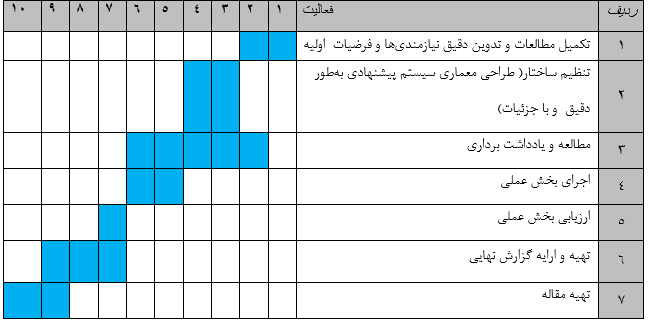
\includegraphics[width=13cm]{figures/Gant.png}
\caption{زمان‌بندی طرح}
\label{Gant}
\end{figure}
\section{امکانات لازم}

 \begin{enumerate}
 \item 	سنسورهای خانه هوشمند(یا توابع شبیه‌سازی سنسورها)
\item 	محیطی جهت برنامه نویسی
\item 	شبکه اینترنت جهت تست
\end{enumerate}
\newpage
\begin{thebibliography}{25}
\begin{LTRbibitems}
\resetlatinfont
\bibitem{M1}
Rosslin John Robles , and Tai-hoon Kim , A Review on Security in Smart Home Development , 2nd ed , International Journal of Advanced Science and Technology
 Vol. 15, February, 2010
 \bibitem{M2}
Jayashri Bangali1 and Arvind Shaligram2,  Design and Implementation of Security Systems for Smart Home based on GSM technology  , 2nd ed , International Journal of Advanced Science and Technology Vol. 15, February, 2013       

\end{LTRbibitems}
\end{thebibliography}
\email{zahra.dehghanian97@gmail.com}
\end{document}
